\section{Verificação dos índices candidatos}
\label{verificacao-custo-indices-candidatos}

A etapa de verificação dos índices candidatos consiste em analisar o custo de execução de todas as consultas avaliadas utilizando cada índice candidato que pode afetar a sua performance. Esta análise de custo é realizada utilizando-se o comando EXPLAIN do MySQL em um banco de dados com todas as tabelas e índices candidatos criados.

O banco de dados utilizado para o processo de verificação dos índices deve ser uma cópia do banco de dados original, com todas as tabelas e dados armazenados. Apenas os índices secundários já existentes devem ser removidos, de forma a não afetar os resultados do otimizador do MySQL durante as execuções das consultas.

Cada índice candidato gerado na etapa anterior é criado no banco de dados individualmente e todas as consultas que são afetadas por ele são avaliadas. Em seguida, o índice é removido do banco de dados e o próximo candidato é avaliado. Este processo se repete até que todos os índices candidatos tenham sido avaliados, conforme ilustrado na figura \ref{fig:verificacao-custo-candidatos}.

\begin{figure}[!hbt]
  \centering
  \caption{Processo de verificação dos índices candidatos.}
  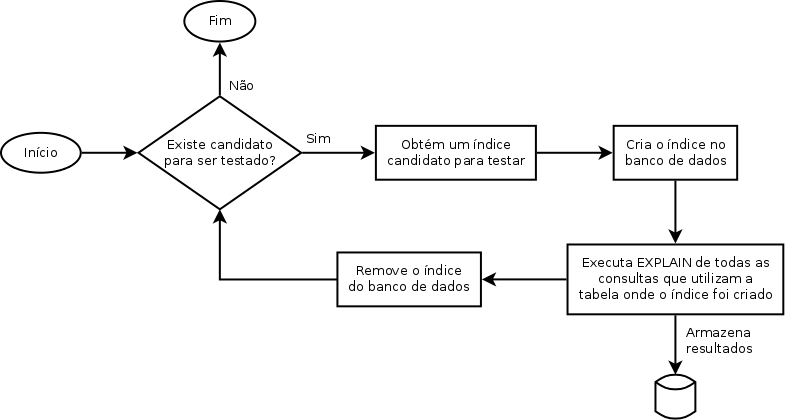
\includegraphics[width=\textwidth]{verificacao-custo-candidatos.png}
  \fonte{Elaborado pelo autor.}
  \label{fig:verificacao-custo-candidatos}
\end{figure}

A avaliação das consultas é realizada através de instruções EXPLAIN, que são enviadas para o servidor do banco de dados MySQL. Para ser possível obter as informações necessárias para o MIST, deve ser utilizada a versão 5.7 ou superior do servidor MySQL. O valor do custo da consulta é retornado pelo servidor MySQL no formato \gls{json}, e é salvo pelo MIST vinculado ao índice utilizado e à consulta verificada. Este valor é utilizado posteriormente para gerar a solução final, como descrito na seção \ref{geracao-solucao-final}.
